% !TEX root = template.tex

\section{Processing Pipeline}
\label{sec:processing_architecture}
The work can be divided in 3 parts: the dataset creation, the neural network creation and the real time prediction.
In order to build an \gls{ars}, a proper dataset was firstly created. All the signals have been divided in several overlapping windows of the same dimension, each window corresponds to a specific activity. The set of windows and the correspondent activity labels created are then divided in training set and test set to learn and assess the prediction model.
The training set is used to fed a \gls{cnn} made by 1D convolutional layers and fully connected layers while the test set is used to assess the accuracy of the learned model and to avoid overfitting problems.

When the \gls{nn} is trained and tested, a new dataset is used in order to verify the effective robustness and generalization of the model in a real time application.
The main steps of the processing pipeline are reported in \fig{fig:processing_pipeline}.

\begin{figure}[htp]
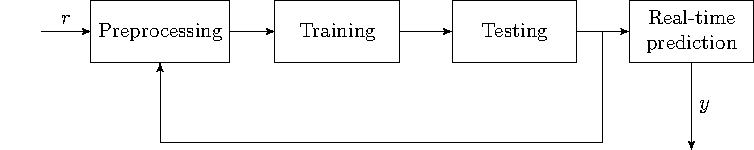
\includegraphics[width=\linewidth]{processing_pipeline}
\caption{Scheme of processing pipeline, $r$ is the raw signal given in input to the preprocessing part, $y$ is the label predicted by the prediction algorithm}
\label{fig:processing_pipeline}
\end{figure}


\section{Signals and Dataset}
\label{sec:model}

\subsection{Measurement setup}
The signals the authors have worked on were provided by \gls{dlr} official website \cite{DLR}. The work is based on the data collected in the datasets  \textit{ARS\_DLR\_Data\_Set\_V2.mat} and \textit{ARS\_DLR\_Benchmark\_Data\_Set.mat}.
Both of them are made up of signals recovered by a \gls{mems} based \gls{imu} (an Xsens MTx-28A53G25) composed by an accelerometer, a gyroscope and a magnetometer. These measurement systems provide information about the inertial acceleration, the angular velocity and the magnetic field direction.
Data are collected recording signals from 14 people while they perform some ordinary motion activities like \textit{standing}, \textit{sitting}, \textit{running}, \textit{jumping}, \textit{lying}. The motion sensor is positioned over the pelvic region of each subject (\fig{fig:IMU}).

\begin{figure}[htp]
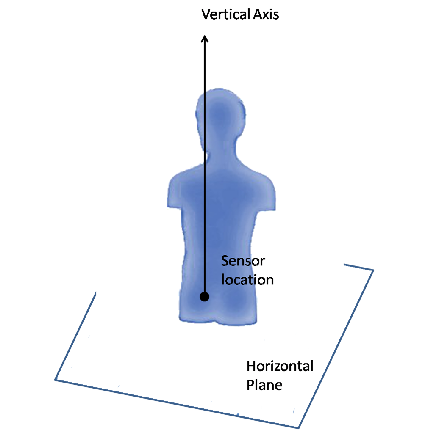
\includegraphics[scale=1.2]{IMU_sensor.pdf}
\caption{Sensor position and the representation of the body frame}
\label{fig:IMU}
\end{figure}

Although the datasets are used in different ways and since they have to comply two different tasks of the \gls{ars}, their structure is exactly the same since their are collected under the same conditions.
Both datasets are divided in activity sessions, 34 in \textit{ARS\_DLR\_Data\_Set\_V2.mat} and 3 in \textit{ARS\_DLR\_Benchmark\_Data\_Set.mat}, each session contains the following field:
\begin{itemize}
\item a matrix of 10 columns in which the first column represents the time domain and the other ones represents the \gls{imu} records over the three sensor axis;
\item a rotation matrix that has the same dimension of the first field and allows to represent the measurement values in the global frame;
\item a vector that contains the activity labels performed during the session (see \tab{tab:label});
\item a vector that indicates when each activity starts and ends.
\end{itemize}

\begin{table}[htp]
\small
	\centering
		\renewcommand{\arraystretch}{1}% Tighter
	\begin{tabular}{@{}lll@{}}
	\toprule
	Label & Index & Description\\ \midrule
	'RUNNING' & $0$ & running \\
	'WALKING' & $1$ & walking \\
	'JUMPING' & $2$ & jumping  \\
	'STNDING' & $3$ & standing \\
	'SITTING' & $4$ & sitting\\
	'XLYINGX' & $5$ & lying \\
	'FALLING' & $6$ & falling \\
	'TRANSUP' & $7$ & getting up i.e.: from sitting to standing \\
	'TRANSDW' & $8$ & going down i.e.: from standing to sitting\\
	'TRNSACC' & $9$ & accelerating\\
	'TRNSDCC' & $10$ & deccelerating\\
	\bottomrule
	\end{tabular}
	\caption{Activities took into consideration with the associated labels}
	\label{tab:label}
\end{table}


\subsection{Signal pre-processing}
The first pre-processing applied to the dataset consists in representing the signals according to the global frame using the rotation matrix. The dataset considered already contains pre-processed data, sampled at T = 0.01s.

In \fig{fig:acc}, \fig{fig:gyr} and \fig{fig:mag} is showed one of Susanna activity sessions. These figures represent the magnitude of accelerometer, gyroscope and magnetometer over the three global axis. Magnitude is plotted instead of the measurements for each axis given the visual meaningfulness of the magnitude, although magnitude is not used in the computation. In particular in \fig{fig:acc} can be noticed the shift of the acceleration's mean around 9.8 $m/s^2$, value coherent with the gravitational constant value \textit{g}. It also emerges in each of these figures how the transitory activities from standing to sitting and vice versa can be seen due to the drastic change of the signals.

Another sort of pre-processing has been made in order to fix the activity indexing of some recordings. It frequently happened to find that, considering two adjacent motion activities, the end of the first activity and the beginning of the second one were not temporarily neighboring. It happened also to find two activities temporarily overlapping: the end of the previous activity was indexed after the beginning of the second one.
The authors resolved the problem removing the non indexed data and the data whose label was uncertain so as to not train the \gls{nn} with wrongly labeled data.

Each session is finally represented as a long and straight matrix with nine columns (three for each measurement system) and a number of rows equals to the session duration.

\begin{figure}[htp]
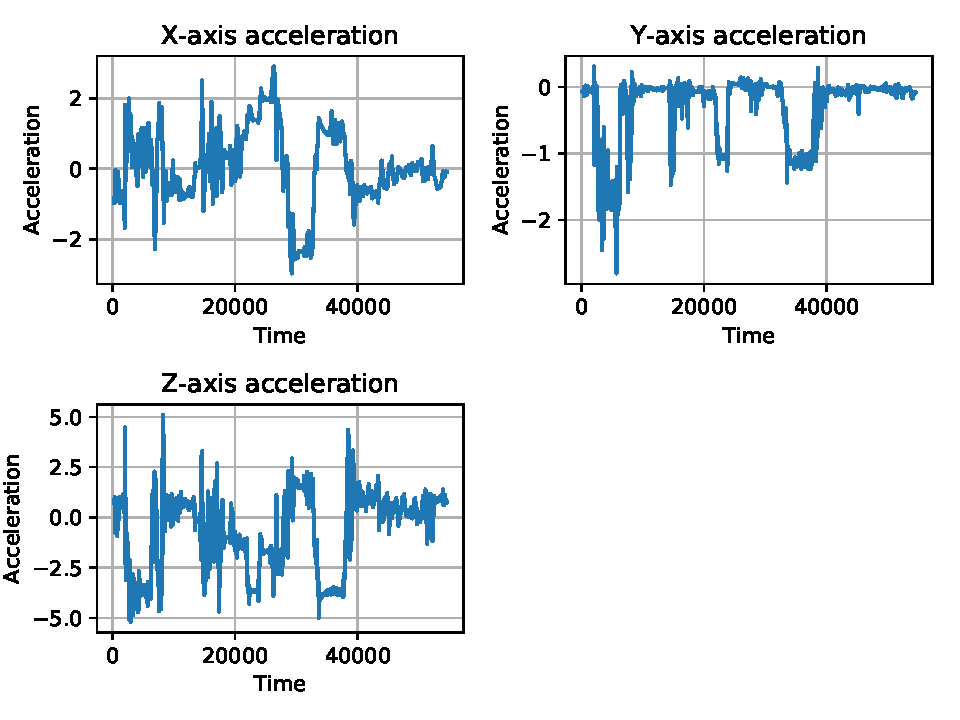
\includegraphics[scale=0.55]{acceleration_susanna.pdf}
\caption{Acceleration norm}
\label{fig:acc}
\end{figure}

\begin{figure}[htp]
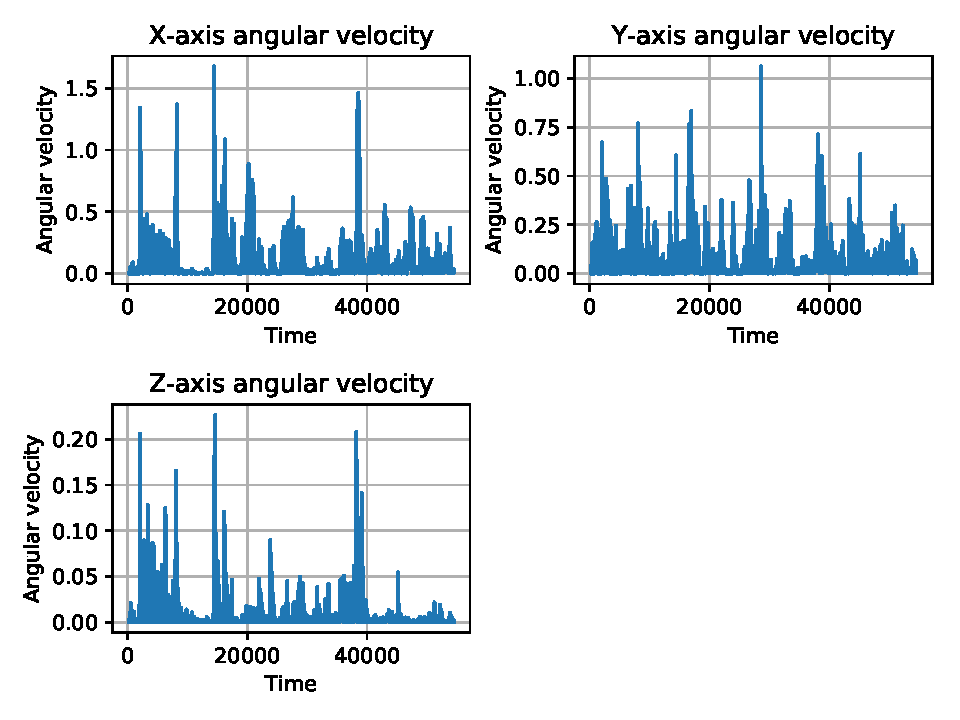
\includegraphics[scale=0.55]{angular_velocity_susanna.pdf}
\caption{Angular velocity norm}
\label{fig:gyr}
\end{figure}

\begin{figure}[htp]
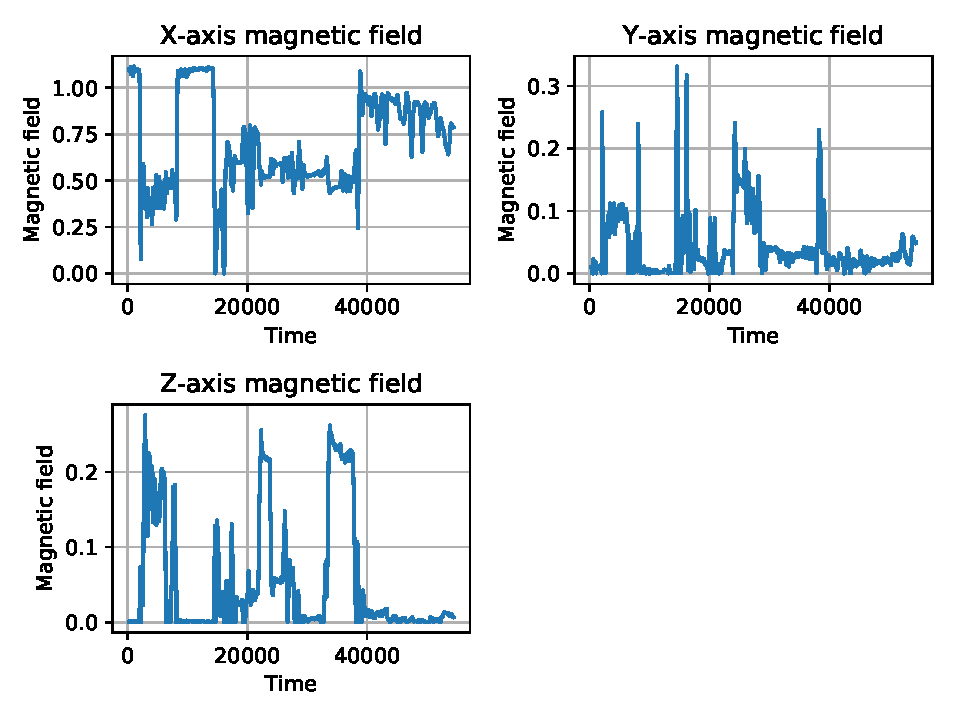
\includegraphics[scale=0.55]{magnetic_field_susanna.pdf}
\caption{Magnetic field norm}
\label{fig:mag}
\end{figure}


\subsection{Dataset creation}

\begin{LaTeXdescription}
	\item[\textit{ARS\_DLR\_Data\_Set\_V2.mat}]
		Since the \gls{cnn} needs a fixed input, each session matrix has been divided in patterns correspondent to a specific activity.
		Every activity, then, has been divided in overlapping windows with stride equals to 3 and length equal to 27 samples, that is the shortest activity length in the whole dataset. The obtained dataset is made by several windows associated to a specific activity label, no transitional windows from an activity to another has been taken. The associated labels are then one hot encoded and, to ensure the independence between an input and the subsequent one in the \gls{cnn}, the dataset is finally shuffled.

	\item[\textit{ARS\_DLR\_Benchmark\_Data\_Set.mat}]
		It is composed by 3 activity sessions and it was used for real time prediction purposes. The signals are segmented in 27 length patterns with stride 5. The algorithm takes into account also transitional windows in order to simulate a realistic real time prediction trial even if they are not considered in the computation of the performance metrics.
\end{LaTeXdescription}


%Even if motion signals are not two dimensional signals, the peculiarity of input shape makes it suitable to be treated as a kind of image with a shape of a vector with 9 channels. Therefore according to the adopted strategy of \textit{Gadaleta et al.}, the dataset was processed in order to be fit into a \gls{cnn} \cite{Gadaleta-2018}.


\section{CNN Architecture}
\label{sec:cnn_architecture}
\begin{figure}[htp]
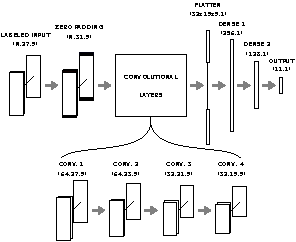
\includegraphics[scale=1.23]{CNN_arch.pdf}
\caption{\gls{cnn} architecture for a single input. Only changing size operations are showed.}
\label{fig:CNN}
\end{figure}


Because of the fixed input shape of the \gls{cnn}, the dataset \MC{which dataset?} is composed by 322502 patterns with shape (27,9) and it was divided in two subsets: the \textit{training set} that is constituted by the 80\% of the whole patterns, the remaining part forms the \textit{testing set}.

The \gls{cnn} architecture is schematically presented in \fig{fig:CNN} and in this section is going to be explained in details using the showed labeling of the layers.

Even if we're working with matrices, we decided to treat the single input pattern as a vertical 27 size vector with 9 channels. Zero Padding was firstly applied at the first and last two rows of the input in order to take in account also the borders in the convolutional layers.

Then four 1D convolutional layers were applied: the changing dimension of a single pattern is shown in \fig{fig:CNN}, the row size is calculated in \tab{tab:filtersize}

\begin{table}[htp]
\small
	\centering
		\renewcommand{\arraystretch}{1}% Tighter
	\begin{tabular}{@{}lllll@{}}
	\toprule
	LAYER & N & K & S & OUTPUT\\
	\midrule
	CONV1 & $31$ & $5$ & $1$ & $(31-5)/1+1 = 27$\\
	CONV2 & $27$ & $5$ & $1$ & $(27-5)/1+1 = 23$\\
	CONV3 & $27$ & $3$ & $1$ & $(23-3)/1+1 = 21$\\
	CONV4 & $21$ & $3$ & $1$ & $(21-3)/1+1 = 19$\\
	\bottomrule
	\end{tabular}
	\caption{Filters dimension along the pattern columns. N is the number of rows of the input pattern. K is the dimension of the kernel. S is the stride dimension.}
	\label{tab:filtersize}
\end{table}

After each convolutional layer is applied a Batch Normalization and a \textit{ReLu} Activation Function.

After this feature learning block follows a classification part made of three fully connected layers:to allow this passage a flattening of Conv4 output filters in necessary (see Flatten layer in \fig{fig:CNN}). Then follows three fully connected layers of size respecively 256, 128 and 11 with a \textit{ReLu} activation function exept except the last one that has a \textit{softmax} function. The last one is the output, each of its 11 elements contains the probability of a label to be the most likely. \textit{Softmax} functions needs to find the label that has the higher probability. Because the \gls{nn} aims to get a classification of more than two labels the loss function used was \textit{categorical crossentropy}.

In order to get a better generalization of the model Dropout layers were added, in particular the authors decided to adopt a dropout of p = 0.15 after Conv1, Conv2 and Conv3, p = 0.25 before Flatten and p = 0.5 after Dense1 and Dense2. This choice was made according to the most commonly used \gls{cnn} configuration proposed by Hinton (p = 0.5 on each fully connected layer) and a more singular configuration proposed by  (p = 0.1-0.2 between the convolutional layers)~\cite{Hinton12}~\cite{Sungheon17}.
The \textit{training set} was trained for 10 epochs with a batch size of 128 and the optimizer used was \textit{adam}.
